\section{Descomposición cíclica, cuarto de giro y momento orientado de Catalán}
\label{iii:sec:catalan}

El registro dodecafásico permite relacionar la respuesta constitutiva con
otros invariantes del transporte. El vínculo se establece sobre subespacios
y aplicaciones determinados: el defecto de rango mide una diferencia de
incidencia, el determinante conserva una respuesta escalar y un coeficiente
del resolvente retiene la orientación. La colección de momentos que culmina
en Catalán interviene a este último nivel.

\subsection{Dos subespacios del ciclo dodecafásico}

En $\mathbb R^{12}$, sea $C e_j=e_{j+1\bmod12}$ y sean
\begin{equation}
 P_3^{\mathrm{cyc}}=\frac{I+C^3+C^6+C^9}{4},\qquad
 P_4^{\mathrm{cyc}}=\frac{I+C^4+C^8}{3},\qquad
 H_d=\operatorname{Ran}P_d^{\mathrm{cyc}}.
 \label{iii:eq:projectors34}
\end{equation}
Los promedios sobre los subgrupos cíclicos son proyectores ortogonales.
$H_3$ está formado por las secuencias periódicas de período divisor de $3$,
y $H_4$ por las de período divisor de $4$. Sus dimensiones son $3$ y $4$.
La restricción de $C$ a cada espacio realiza el ciclo correspondiente.
El superíndice $\mathrm{cyc}$ identifica el promedio del ciclo dodecafásico:
$P_3^{\mathrm{cyc}}$ es el proyector sobre las secuencias de período divisor
de $3$. Su dominio y su acción son distintos de los del proyector isótipo
tridimensional de la realización icosaédrica; la coincidencia de rango
no identifica ambos operadores.

\begin{proposition}[Defecto de rango y respuesta determinantal]
Se verifican
\begin{equation}
 \frac{\operatorname{Tr}(P_3^{\mathrm{cyc}}-P_4^{\mathrm{cyc}})}{12}=-\frac1{12},\qquad
 \frac{\det_{H_3}(I-sC)}{\det_{H_4}(I-sC)}
 =\frac{1-s^3}{1-s^4}=f(s),\quad 0<s<1.
 \label{iii:eq:trace-det}
\end{equation}
\end{proposition}
\begin{proof}
La traza de un proyector ortogonal es su rango, de modo que el numerador
de la primera expresión es $3-4$. El polinomio característico de un ciclo
de longitud $d$ es $t^d-1$; por ello su determinante $\det(I-sC)$ es
$1-s^d$. El cociente produce la segunda identidad.
\end{proof}

La sustitución $s=q^{30}$ transporta esta representación al cociente
$90/120$. En $s=1$, el modo constante común se cancela antes de tomar el
límite, que vale $3/4$. Esta realización de $-1/12$ como defecto de traza
tiene un dominio finito explícito. Las realizaciones regularizadas y
modulares del mismo escalar conservan sus operadores y dominios propios.

\subsection{Representación fiel del cuarto de giro}

Definamos el proyector antipodal $P_{\rm ant}=(I-C^6)/2$ y
$Q=P_4^{\mathrm{cyc}}P_{\rm ant}$. Este proyector actúa sobre el ciclo de doce fases y es
distinto del proyector constitutivo $P_-$ de la sección~\ref{iii:sec:constitutiva}.
Los proyectores $P_4^{\mathrm{cyc}}$ y $P_{\rm ant}$ conmutan y
$Q$ tiene rango $2$. En su imagen se fija la base ortonormal
\begin{equation}
 u=\frac1{\sqrt6}(1,0,-1,0,1,0,-1,0,1,0,-1,0)^{\mathsf T},
 \qquad v=Cu.
 \label{iii:eq:uv}
\end{equation}
Se comprueba componente a componente que $Cu=v$ y $Cv=-u$. En consecuencia,
la isometría $W(a,b)=au+bv$ satisface
\begin{equation}
 CW=WJ,\qquad
 J=\begin{pmatrix}0&-1\\1&0\end{pmatrix},\qquad J^2=-I.
 \label{iii:eq:quarter-intertwiner}
\end{equation}
La estructura compleja del plano queda realizada por la acción efectiva del
ciclo. El signo depende de la orientación fijada: en la misma base,
$C^3W=-WJ$. Esta precisión permite componer el plano con el lector orientado.

\subsection{Resolvente y profundidad ilimitada}

Como $C^2=-I$ sobre $\operatorname{Ran}Q$, para $0\leq s<1$ se tiene
\begin{equation}
 (I-sC)^{-1}\big|_{\operatorname{Ran}Q}=\frac{I+sC}{1+s^2},
 \qquad k_4(s):=\langle v,(I-sC)^{-1}u\rangle=\frac{s}{1+s^2}.
 \label{iii:eq:resolvent}
\end{equation}
La sucesión $\langle v,C^nu\rangle$ es $0,1,0,-1,\ldots$. El lector
de profundidad conserva este carácter mediante el momento
\begin{equation}
 \mathcal C_2(s)=\sum_{k\geq0}\frac{(-1)^ks^{2k+1}}{(2k+1)^2},
 \qquad 0\leq s\leq1.
 \label{iii:eq:c2}
\end{equation}
La serie converge absolutamente y uniformemente en ese intervalo por
comparación con $\sum(2k+1)^{-2}$. Para $0<s<1$, las series derivadas
convergen uniformemente sobre cada intervalo compacto interior. Con
$\mathcal D=s\,d/ds$, se obtiene
\begin{equation}
 \mathcal D^2\mathcal C_2(s)=k_4(s),\qquad
 \mathcal C_2(s)=\int_0^s\frac{dt}{t}\int_0^t\frac{d\xi}{\xi}\,k_4(\xi).
 \label{iii:eq:c2-integral}
\end{equation}
Las condiciones $\mathcal C_2(0)=0$ y
$\lim_{s\downarrow0}\mathcal D\mathcal C_2(s)=0$ fijan las dos constantes
de integración. En efecto, la diferencia de dos soluciones de
$\mathcal D^2F=k_4$ tiene la forma $a\log s+b$; la segunda condición
anula $a$ y la primera anula $b$.
La convergencia uniforme permite evaluar el extremo $s=1$: el resultado es
el momento de Catalán. La representación finita del carácter conserva su
orientación; el índice de profundidad permanece ilimitado.

\subsection{Composición con la respuesta constitutiva}

\begin{theorem}[Relación diferencial constitutiva]
Para $0<s<1$, con la orientación de \eqref{iii:eq:uv},
\begin{equation}
 f(s)=\frac{1+s+s^2}{s(1+s)}\,\mathcal D^2\mathcal C_2(s).
 \label{iii:eq:catalan-vacuum}
\end{equation}
\end{theorem}
\begin{proof}
Sustituir \eqref{iii:eq:resolvent} en \eqref{iii:eq:c2-integral} y utilizar
$(1+s)(1+s^2)=1+s+s^2+s^3$ da la identidad. Todos los denominadores son
positivos en el dominio. El entrelazador \eqref{iii:eq:quarter-intertwiner}
identifica el coeficiente operatorio utilizado antes de su evaluación.
\end{proof}

Al evaluar $s_\pm=q_\pm^{30}$, la misma colección produce las dos respuestas
de canal de \eqref{iii:eq:rchannels}. El límite de Catalán, el defecto de
traza y los autovalores constitutivos mantienen sus funciones diferentes
dentro de esta composición. La inversión del ciclo con las marcas $u,v$
fijas cambia el signo de $k_4$ y conserva el determinante $1+s^2$.
Así se identifica una información de orientación que el determinante
aislado no distingue.

El desarrollo de Pell utiliza una evaluación particular de esta colección,
con $\rho=2-\sqrt3$ y $\rho^{-1}=2+\sqrt3$. Su prueba se conserva como
unidad propia de integración; la definición angular de $q_\pm$ permanece
independiente de una eventual identificación de $s_\pm$ con $\rho$.

La figura~\ref{iii:fig:respuesta-momento-pell} representa la relación entre
la respuesta racional y el núcleo orientado antes de integrar. La sección
de Pell satisface $\rho+\rho^{-1}=4$, por lo que
$k_4(\rho)=(\rho+\rho^{-1})^{-1}=1/4$. Los dos valores constitutivos
se obtienen, en cambio, evaluando $f$ en los argumentos $s_\pm$ ya
construidos. El trazado incluye las prolongaciones continuas de las dos
funciones a $[0,1]$; el dominio de inversión constitutiva sigue siendo
el intervalo abierto $(0,1)$.

\begin{figure}[htbp]
\centering
\begin{tikzpicture}[x=10cm,y=4.6cm,>=stealth]
 \pgfmathsetmacro{\pellrho}{2-sqrt(3)}
 \pgfmathsetmacro{\fpell}{(1+\pellrho+\pellrho^2)/(1+\pellrho+\pellrho^2+\pellrho^3)}
 \draw[gray!35,thin] (0,0.25)--(1,0.25);
 \draw[gray!35,thin] (0,0.5)--(1,0.5);
 \draw[gray!35,thin] (0,0.75)--(1,0.75);
 \draw[gray!35,thin] (0,1)--(1,1);
 \draw[->] (0,0)--(1.04,0) node[right] {$s$};
 \draw[->] (0,0)--(0,1.1) node[above] {valor adimensional};
 \foreach \xx/\lab in {0/0,0.5/{1/2},1/1}{
  \draw (\xx,0)--(\xx,-0.015) node[below] {$\lab$};
 }
 \foreach \yy/\lab in {0.25/{1/4},0.5/{1/2},0.75/{3/4},1/1}{
  \draw (0,\yy)--(-0.008,\yy) node[left] {$\lab$};
 }
 \draw[gray!70,densely dashed] (\pellrho,0)--(\pellrho,1.035);
 \node[below,align=center,font=\small] at (\pellrho,-0.015)
  {$\rho$\\[-1pt]$2-\sqrt3$};
 \draw[black,very thick,domain=0:1,samples=121,smooth]
  plot (\x,{(1+\x+\x^2)/(1+\x+\x^2+\x^3)});
 \draw[blue!65!black,thick,dashed,domain=0:1,samples=121,smooth]
  plot (\x,{\x/(1+\x^2)});
 \fill[black] (\pellrho,\fpell) circle[radius=1.7pt];
 \fill[blue!65!black] (\pellrho,0.25) circle[radius=1.7pt];
 \node[anchor=south west,font=\small,fill=white,inner sep=2pt] at (0.51,0.94)
  {$f(s)=\dfrac{1+s+s^2}{1+s+s^2+s^3}$};
 \node[anchor=south west,text=blue!65!black,font=\small] at (0.57,0.55)
  {$k_4(s)=\dfrac{s}{1+s^2}$};
 \node[anchor=north west,font=\small,fill=white,inner sep=2pt]
  at (0.30,0.225) {$k_4(\rho)=1/4$};
\end{tikzpicture}
\caption{Respuesta constitutiva y núcleo del momento orientado. La curva
continua es $f$ y la discontinua es
$k_4=\mathcal D^2\mathcal C_2$; ambas se relacionan mediante
\eqref{iii:eq:catalan-vacuum}. La recta vertical marca la sección de Pell,
sin identificarla con los argumentos constitutivos $s_+$ o $s_-$.}
\label{iii:fig:respuesta-momento-pell}
\end{figure}
